\documentclass[a4paper]{article}
\usepackage{amsmath}
\usepackage{amsfonts}
\usepackage{amssymb}
\usepackage{graphicx}
\usepackage{booktabs} 
\usepackage{hyperref}
\usepackage{geometry}
\usepackage{caption}
\usepackage{float}
\usepackage{array}
\usepackage{xcolor}
\usepackage[edges]{forest}
\usepackage{multicol}

\newcommand{\code}[1]{\colorbox{gray!20}{\texttt{#1}}}

\begin{document}

\begin{titlepage}
    \vspace*{2cm}
    \begin{center}


    \begin{figure}
    \centering
        
\includegraphics[width=0.6\linewidth]{unilogo.png}
    \end{figure}

    \vspace*{2cm}

    \LARGE

    \textbf{LLM Benchmark project Report}


    \vspace{3.5cm}
    \normalsize
    \begin{minipage}[t]{0.47\textwidth} 
        {Professors:} \vspace{0.3em} \\
        {\large \textbf{Michele Lombardi}} \vspace{1em}\\
        {\large \textbf{Allegra De Filippo}}
    \end{minipage}
    \hfill
    \begin{minipage}[t]{0.47\textwidth}\raggedleft
    {Students:} \hspace{-0.9em} \vspace{0.3em} \\
        {\large \textbf{Simone Migliaccio (matr.: 0001159303)}}\vspace{0.2em}\\
        {\large \textbf{Simone Spezia (matr.: 0001167605)}}\vspace{0.2em}\\
        {\large \textbf{Alberto Varini (matr.: 0001189363)}}\\
    \end{minipage}

    \end{center}

\end{titlepage}

\newgeometry{top=3cm, bottom=3cm, left=3cm, right=3cm}
\tableofcontents
\newpage

\section{Introduction}
The main goal of this project is to provide a general benchmark to evaluate different LLMs performances under different types of planning domains to better understand in advance what are the planning capabilities of a given LLM. In the following sections the main features of this projects are going to be shown.\\
Also a quick PDDL starting guide has been created to better gain the necessary knowledge about PDDL this specific language used to define planning problems.

\section{General Structure}
The root folder contains various sub folders, specifically:
\begin{itemize}
    \item analysis
    \item archive
    \item Benchmark Framework
    \item results
\end{itemize}

\subsection{Benchmark Framework structure}
The folder Benchmark Framework is the core of all the work we've done. The main goal of this framework was to provide a easy to use and general testing platform to be employed when evaluating the performances of a LLM is needed, 
The following pages are going to be used to show the folders and the structure of the framework:
\vspace{0.2cm}
\begin{center}
        

    \begin{forest} 
            for tree={
                font=\ttfamily\footnotesize,
                grow'=0,
                child anchor=west,
                parent anchor=south,
                anchor=west,
                calign=fixed edge angles,
                edge={draw, semithick},
                l sep = 7pt,       % Ridotto lo spazio orizzontale tra i livelli
                s sep = 3pt,       % Ridotto lo spazio verticale tra le cartelle
                inner sep = 2.5pt,  % ridotto spazio attorno al testo
                folder, % stile cartella
            }
            [LLM Benchmark/
                [docs/]
                [evaluators/]
                [Leonardo script/]
                [models/]
                [outputs/]
                [prompts/]
                [protocols/]
                [reporting/]
                [runner/]
                [scripts/]
                [slurm logs/]
                [tasks/]
                [tests/]
                [utils/]
                [advanced planning evaluation.py]
                [clear outputs-py]
                [run benchmark.py]
                [setup.md]
            ]
            \end{forest}
\end{center}

\paragraph{run benchmark} 
quesgto è la sezione in cyui si spiega run benchmark


\section{PDDL Problems Classification}
The first thing to do since we wanted a trustable benchmark and since a lot of PDDL models were already provided as reference material was to classify the problems 
using a numerical difficulty score. We used a numerical score because it is intuitively understandable by anyone who will ever want to compare the performance of 
LLMs using these models.
Another classification implemented consists into separating problems in different categories based on the type of reasoning they request.
To compute the scores the code can be found in the file \texttt{score\_domains\_complexity.py}

    \subsection{Difficulty Classification}
    \subsubsection{Instances scores}
    The complexity of a single problem instance is calculated using a weighted logarithmic combination of four key metrics. The use of the logarithm prevents any single feature from dominating the score excessively.\\

    The \textbf{Raw Score} is defined as:
    \begin{equation}
        Raw\_score = 0.45 \cdot \log(1 + A) + 0.20 \cdot \log(1 + G) + 0.20 \cdot \log(1 + N) + 0.15 \cdot T
    \end{equation}

    Where:
    \begin{itemize}
        \item \textbf{A (Actions):} Number of feasible grounded actions. This is estimated by unifying action parameters with objects that satisfy static preconditions in the initial state.
        \item \textbf{G (Goals):} Total number of atomic conditions in the goal state.
        \item \textbf{N (Numeric Score):} A composite value representing numeric complexity:
        \begin{equation}
            N = E_{num} + 2 \cdot P_{num} + 3 \cdot G_{num} + M
        \end{equation}
        where $E_{num}$ are numeric effects, $P_{num}$ numeric preconditions, $G_{num}$ numeric goal conditions, and $M$ is a binary flag for the presence of a metric.
        \item \textbf{T (Topology Score):} Evaluates the spatial/relational complexity based on predicates like \textit{adj} or \textit{connected}:
        \begin{equation}
            T = \log(1 + Nodes) + \log(1 + Edges) + Density
        \end{equation}
    \end{itemize}
    Obviously a different weight could be assigned to each different part of the computation of raw scores depending on the operator that is doing the tests in order to higlight more for example the number of action present in the instances and so on.\\
    Finally, an \textbf{Instance Score (0-100)} is calculated by normalizing the raw score relative to the minimum and maximum scores found within the same domain. The results can be found in the folder \texttt{domains\_complexity}.\\
    Note that also some additional statistics for each domain are computed based on the results obtained from the instances, for example it could be of interest evaluating the mean and the median of the scores obtain form the instances of a single domain.

    \subsubsection{Domain scores}
    The overall difficulty of a domain is not just the average of its instances, but a reflection of its total state-space and constraint complexity.
    The \textbf{Domain Difficulty (0-100)} is computed by:
    \begin{enumerate}
        \item Summing the $S_{raw}$ of all instances belonging to the domain to obtain a \textit{Total Raw Score}.
        \item Normalizing this total across all tested domains in the benchmark.
    \end{enumerate}
    This approach ensures that a domain with many complex instances is ranked higher than one with few simple instances, note that obviously the easiest problems gets a domain difficulty equal to 0 (in this case is the "fo-sailing" problem) and the problem with the highest difficulty has domain difficulty equal to 100, (in our case the "settlersnumeric" problem).

    \subsubsection{Results obtained}
    In order to obtain a visual representation of the classified problems, we produced heatmaps for both the overall normalized domain scores and the raw scores.
    \begin{figure}[H]
    \centering
        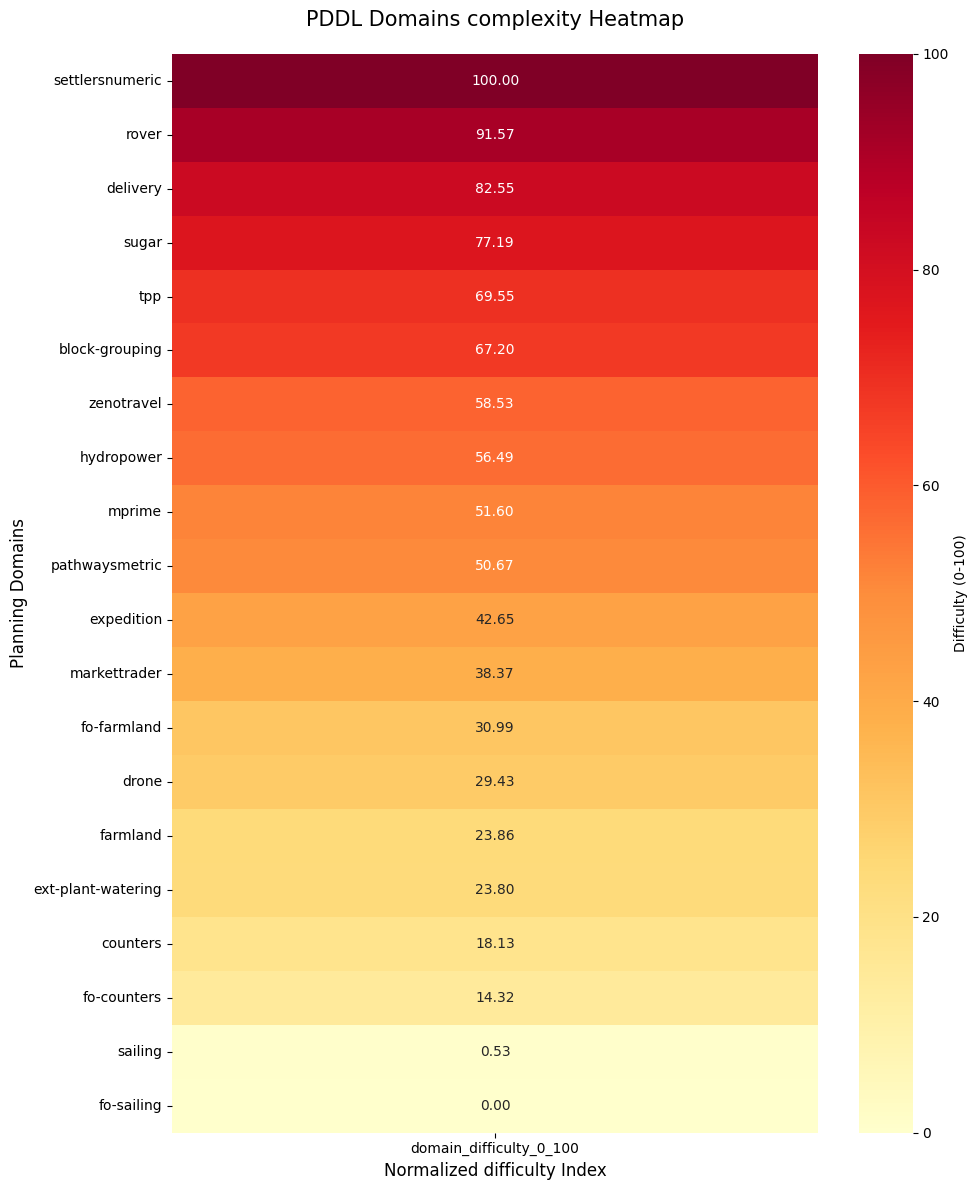
\includegraphics[width=0.6\linewidth]{domaincompl.png}
    \end{figure}

    \begin{figure}[H]
    \centering
        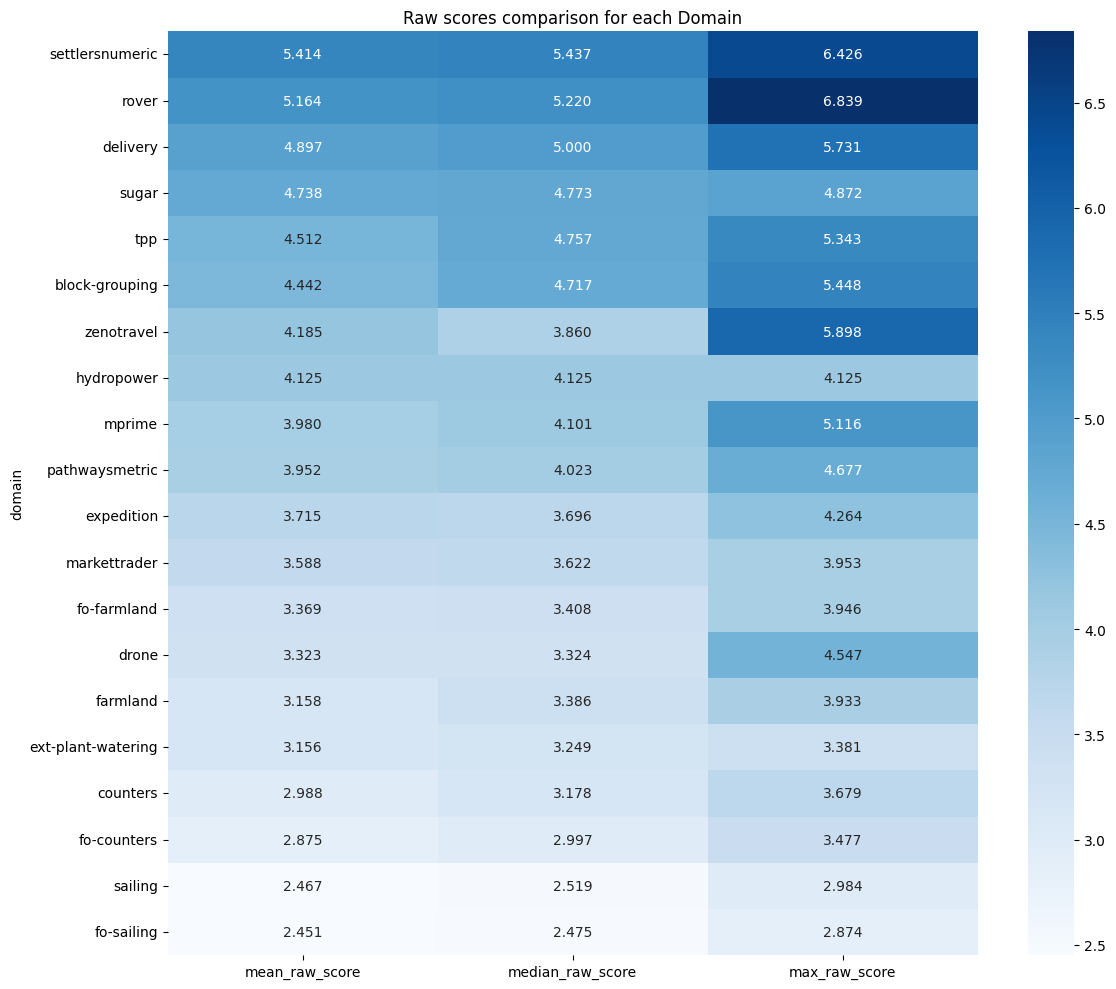
\includegraphics[width=0.6\linewidth]{rawscoreshm.png}
    \end{figure}

    
    \subsection{Reasoning Classification}
    Here the classification based on the type of reasoning these problems require the LLM to employ is shown. We decided to split the reasoning types into 5 categories:
    \begin{itemize}
        \item \textbf{Spatial:} These problems are typically about objects that have to be moved in a 2D (or more dimensional) spaceframe.
        \item \textbf{Numerical Optimization:} These problems require from the LLM an extensive capacity to deal with numerical optimization problems, such as managing complex cost functions and resource constraints.
        \item \textbf{Temporal Planning:} In this kind of problem it is required from the LLM to be able to reach the goal defining an order between objects having timing constraints and relations.
        \item \textbf{Logistic:} In this kind of problems it is required to reach the goal by planning some kind of goods transportation and agents coordination.
        \item \textbf{Logic:} These are abstract puzzles where the state space and actions represent symbolic or mathematical transformations rather than physical interactions. They test the model's ability to reason over purely formal rules without relying on world knowledge.
    \end{itemize}

    In the following table the classification of the 20 planning problems is shown, note that in this case all the work have been done by hand and that the problems in the table are ordered form hardest to easiest following the previous difficulty classification. Note also that the evaluation is based on how much the problem belong to the specific domain, for example in the problem "settlersnumeric" there is a dominant Numerical Optimization part hence the problem is going to be classified as a Numerical Optimization problem.
    
    \begin{table}[H]
        \centering
        \renewcommand{\arraystretch}{1.25} 
        
        \begin{tabular}{c|c}
            \toprule
            
            \textbf{PDDL Problem} & \textbf{Reasoning Category} \\
            
            \midrule[1pt]
            \addlinespace[0.25cm]
            Settlersnumeric & Numerical Optimization \\
            \midrule
            Rover & Logistic \\
            \midrule
            Delivery & Logistic \\
            \midrule
            Sugar & Numerical Optimization \\
            \midrule
            Tpp & Numerical Optimization \\
            \midrule
            Block-Grouping & Spatial \\
            \midrule
            Zenotravel & Logistic \\
            \midrule
            Hydropower & Temporal Planning \\
            \midrule
            Mprime & Logic \\
            \midrule
            Pathwaysmetric & Numerical Optimization \\
            \midrule
            Expedition & Logistic \\
            \midrule
            Markettrader & Numerical Optimization \\
            \midrule
            Fo-farmland & Numerical Optimization \\
            \midrule
            Drone & Spatial \\
            \midrule
            Farmland & Numerical Optimization \\
            \midrule
            Ext-Plant-Watering & Spatial \\
            \midrule
            Counters & Numerical Optimization \\
            \midrule
            Fo-Counters & Numerical Optimization \\
            \midrule
            Sailing & Spatial \\
            \midrule
            Fo-Sailing & Spatial \\
            
        \end{tabular}
        \vspace{0.2cm}
        \caption{Reasoning Category Classification Tab}
        \label{tab:dati_pfile_griglia}
    \end{table}

    \subsection{Problems chosen}
    In order to chose the correct problem to be solved by LLMs we decided to pick 3 sets composed by 3 problems each. The sets are composed by 3 problems with different reasoning categories and specifically from the categories Numericaal Optimization, Spatial and Logistic. Problems related to Temporal Planning and Logic were not chosen since just one problem for each type was present; we suggest, in order to study the capabilities of LLMs in these domains, to use a PDDL problenms dataset specifically containing these kind of problems.\\
    In order to better understand how we picked the problems the following tables are shown, the elements are ordered with decreasing difficulty.
    
    \begin{table}[H]
    \centering
    \renewcommand{\arraystretch}{1.5} 

    % --- PRIMA TABELLA ---
    % 0.31\textwidth significa che occupa il 31% della larghezza della pagina
    \begin{minipage}[t]{0.31\textwidth}
        \centering
        \begin{tabular}[t]{ >{\centering\arraybackslash}p{0.9\linewidth} }
            \toprule
            \textbf{Numerical Optimization}\\
            \midrule[1pt]
            \addlinespace[0.15cm]
            Settlersnumeric\\
            \midrule
            Sugar\\
            \midrule
            Tpp\\
            \midrule
            Pathwaysmetric\\
            \midrule
            Markettrader\\
            \midrule
            Fo-farmland\\
            \midrule
            Farmland\\
            \midrule
            Counters\\
            \midrule
            Fo-Counters\\
            \bottomrule
        \end{tabular}
    \end{minipage}%
    \hfill % <--- TRUCCO: Inserisce uno spazio elastico automatico tra le tabelle
    % --- SECONDA TABELLA ---
    \begin{minipage}[t]{0.31\textwidth}
        \centering
        \begin{tabular}[t]{ >{\centering\arraybackslash}p{0.9\linewidth} }
            \toprule
            \textbf{Spatial}\\
            \midrule[1pt]
            \addlinespace[0.15cm]
            Block-Grouping\\
            \midrule
            Drone\\
            \midrule
            Ext-Plant-Watering\\
            \midrule
            Sailing\\
            \midrule
            Fo-Sailing\\
            \bottomrule
        \end{tabular}
    \end{minipage}%
    \hfill % <--- Altro spazio elastico automatico
    % --- TERZA TABELLA ---
    \begin{minipage}[t]{0.31\textwidth}
        \centering
        \begin{tabular}[t]{ >{\centering\arraybackslash}p{0.9\linewidth} }
            \toprule
            \textbf{Logistic}\\
            \midrule[1pt]
            \addlinespace[0.15cm]
            Rover\\
            \midrule
            Delivery\\
            \midrule
            Zenotravel\\
            \midrule
            Expedition\\
            \bottomrule
        \end{tabular}
    \end{minipage}

    \vspace{0.4cm}
    \caption{Reasoning Categories Selected for Benchmark}
    \label{tab:tre_tabelle_affiancate}
\end{table}
In order to obtain a more clear output from the LLM we decided to select two differents sets of three problems each and specifically:
\begin{itemize}
    \item \textbf{Hard Set:} composed by \textit{settlersnumeric, block-grouping, rover}

    \item \textbf{Easy Set:} composed by \textit{fo counters, fo sailing, expedition}
\end{itemize}
It is clearly visible that we picked respectively the most three difficult problems and the three easiest ones. This has been done to ensure also in the outputs a visible difference in the metrics when evalauting the outputs.\\
Additionally it can be seen from the following heatmap that the instances of these domains have increasing difficulty:
    \begin{figure}[H]
    \centering
        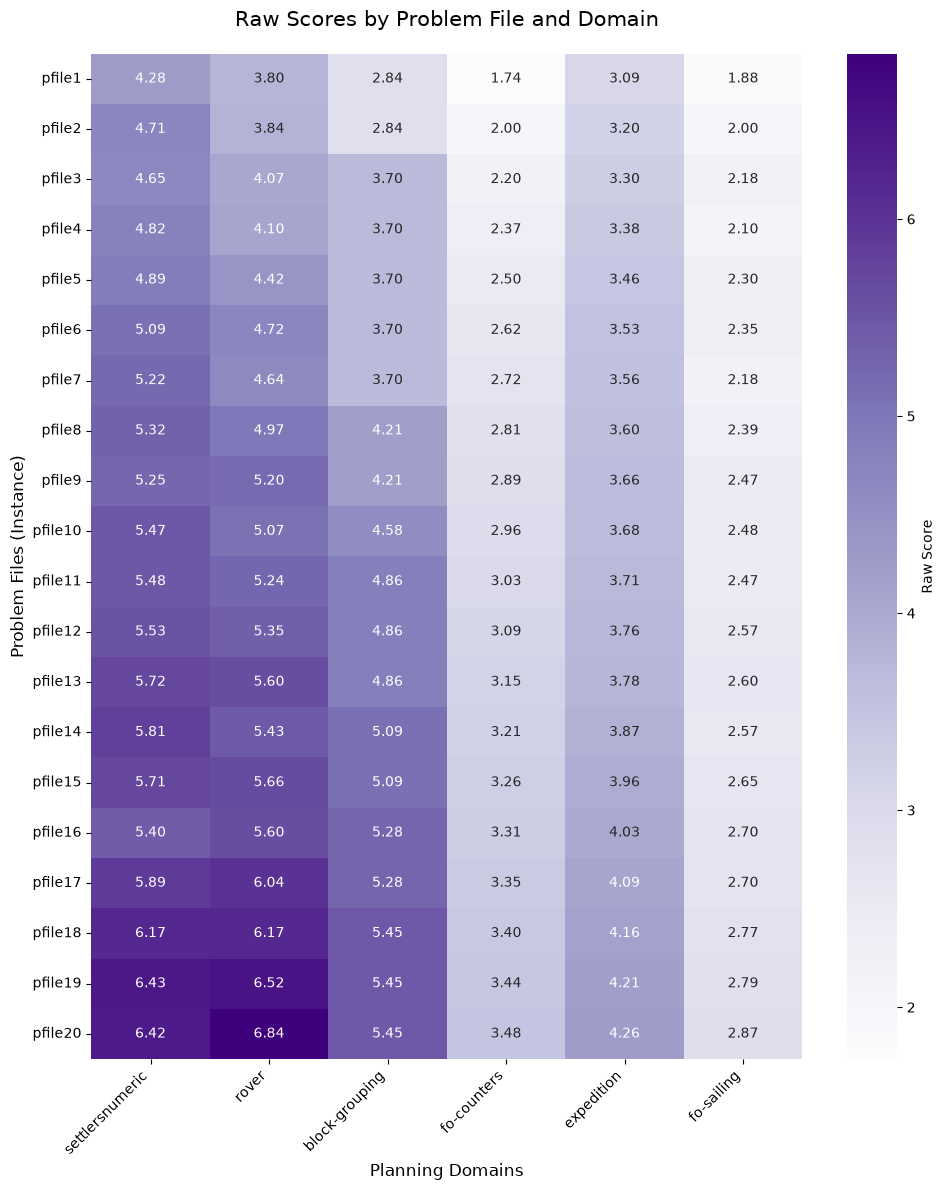
\includegraphics[width=0.6\linewidth]{Instances.png}
    \end{figure}
It is clearly visible both the difference in terms of difficulty between the Hard set and the Easy set and the increasing difficulty related to the pfiles; because of this last consideration we applied an additional, partition to divide the pfiles in three different categories and specifically:
\begin{itemize}
    \item Easy (composed by pfiles from 1 to 4)
    \item Medium (composed by pfiles from 8 to 11)
    \item Hard (composed by pfiles from 15 to 18)
\end{itemize}
Also it is worth noticing that we did not use all the instances available for each selected domain but we decided to choose a small batch (4 instances) of instances representing the easy, medium and hard categories.


\section{LLMs Models Implemented}
In this section the LLMs models chosen to solve the problems as well as the reason behind aforementioned choice are going to be detailed. The reasons behind the choice of the LLms are basically two: 
\begin{itemize}
    \item The hardware platform available
    \item The release date of the LLMs
\end{itemize}
In order to obtain a wider range of outputs 5 LLMs were chosen and downloaded by Huggingface, the specific models and versions used are going to be explored later on.

    \subsection{Hardware platform}
    Before listing the LLMs models chosen it is worth saying that we used a cluster from Leonardo HPC by Cineca consisting n
        \subsubsection{notes on nvidia API}
        ????

    \subsection{Release time}

    \subsection{Models chosen}






\section{Benchmark output Parsing and Output Structure}
\textcolor{red}{\LARGE\MakeUppercase{DA RIEMPIRE}}

\section{Output Validation Using VAL}
\textcolor{red}{\LARGE\MakeUppercase{DA RIEMPIRE}}

\section{LLMs Reasoning Capabilities Evaluation}
    \subsection{Pipeline and Data flow}
    How Raw / Parsed / Scored become one DataFrame , which Classes hold the state the metrics need and why the load $\rightarrow$ row $\rightarrow$ aggregate $\rightarrow$ plot $\rightarrow$ report stages.
    This section maps the analysis script \texttt{advanced\_planning\_evaluation\_sp.py} onto the rest of the Repo , showing how the three on-disk artifact layers Raw / Parsed / Scored.
    become DataFrames , which data classes exist and why and how the data-manipulation stage hands off to metric computation and visualization.
        \subsubsection{Pipeline Generic description}
        Everything funnels into one DataFrame \code{df\_metrics} , which is the single source of truth for every groupby and every plot.
        we start from the outputs:
        \begin{itemize}
            \item raw\ : generation text + reasoning text
            \item parsed\ : raw.actions + reasonig.actions
            \item scored\ : VAL outputs solved , prefix lenght , valid@k informations
            \item tasks\ : domain.pddl + pfileN.pddl
        \end{itemize}
        
        \code{look\_artifact\_rows()} takes the data present in Parsed and then joins Raw and Scored data in a single row for each instance , collapsing the retry loop by scanning the attemps back to front keeping the last non empty plan as the representative \code{\_actions} , while preserving the full attemp list \code{\_parsed\_attemps},\code{\_scored\_attemps}, \code{\_raw\_attemps} as private colums so per-iteration metrics can still be computed downstream.
        Keeping the grain at instance level leads to every aggregate metric (SR , HR , PS ) bein an average over comparable units , while maintaining the iteration structure in the private \code{\_*\_attemps} and used as option by the metrics that explicitly need it like (FASR , IWSR , iteration profile , CoTal ).
        For each row is also added Validity and Iteration count taken from the Scored file \code{Valid = scored["solved"] , Iterations = scored["iterations\_used"]}, the presence of the CoT is instead taken from \code{\string\protocols\string\protocol.yaml} or instead as a fallback is looked the presence of reasonig actions or text since we want to compute the Cot alignement metric only for those models that have it available.
        this function resites for each row the \code{df\_raw} informations:
        \begin{itemize}
            \item Model
            \item Domain
            \item Problem
            \item Difficulty
            \item Protocol
            \item Run\_id
            \item Valid
            \item Length
            \item Iterations
            \item Chain\_of\_Thought
            \item actions
            \item \_cot\_text
            \item \_parsed\_attempts
            \item \_scored\_attempts
            \item \_raw\_attempts
            \item \_file\_path
            \item parsed\_file\_path
            \item iterations 
        \end{itemize}
    \subsection{Metrics scientific foundation}
    \subsection{Metric Families}
        \subsubsection{Planning Efficiency}
        \subsubsection{Execution and Reasoning}
        \subsubsection{Grounding and Discriminatory}
        \subsubsection{PS (Composite Planning Score)}
    \subsection{Cross-Domain and Cross-LLM comparison}


\section{Conclusions}
\textcolor{red}{\LARGE\MakeUppercase{DA RIEMPIRE}}


\end{document}